\documentclass[11pt,a4paper]{article}

\usepackage[margin=2.35cm]{geometry}
\usepackage[T1]{fontenc}
\usepackage[utf8]{inputenc}
\usepackage[english]{babel}
\usepackage{lmodern}
\usepackage{microtype}
\usepackage{csquotes}
\usepackage{graphicx}
\usepackage{xcolor}
\usepackage{booktabs}
\usepackage{array}
\usepackage{tabularx}
\usepackage{longtable}
\usepackage{float}
\usepackage{placeins}
\usepackage{enumitem}
\usepackage{amsmath}
\usepackage{amssymb}
\usepackage[hidelinks]{hyperref}
\usepackage{caption}
\usepackage{fancyhdr}
\usepackage[backend=biber,style=numeric,sorting=none,maxbibnames=99,url=false,doi=true,eprint=true]{biblatex}
\addbibresource{references.bib}
\AtBeginBibliography{\small}

\definecolor{accent}{RGB}{37,78,118}
\definecolor{lightgray}{RGB}{245,247,249}
\hypersetup{
  colorlinks=true,
  linkcolor=accent,
  citecolor=accent,
  urlcolor=accent,
  pdftitle={Context Aware Stress Testing of Visual Explanations in Multimodal Large Language Models},
  pdfauthor={Lorenzo Castellano},
  pdfsubject={Prompt Ablation with Token Activation Maps},
  pdfkeywords={MLLM, explainability, Token Activation Maps, prompt sensitivity, Qwen2-VL}
}

\setlength{\parindent}{0pt}
\setlength{\parskip}{0.55\baselineskip}
\setlist[itemize]{topsep=0.25em,itemsep=0.15em,leftmargin=1.4em}
\setlist[enumerate]{topsep=0.25em,itemsep=0.15em,leftmargin=1.6em}
\captionsetup{font=small,labelfont=bf}
\renewcommand{\arraystretch}{1.12}
\newcolumntype{Y}{>{\raggedright\arraybackslash}X}
\newcolumntype{Z}{>{\raggedright\arraybackslash}p{0.28\linewidth}}
\newcommand{\code}[1]{\texttt{\small #1}}
\newcommand{\prompt}[1]{\texttt{\footnotesize #1}}

\pagestyle{fancy}
\fancyhf{}
\lhead{Context aware stress testing of visual explanations}
\rhead{Lorenzo Castellano}
\cfoot{\thepage}
\setlength{\headheight}{14pt}

\begin{document}
\pagenumbering{gobble}

\begin{titlepage}
\centering
\vspace*{2.5cm}
{\Large CASA Project Report\par}
\vspace{1.1cm}
{\huge\bfseries Context Aware Stress Testing of Visual Explanations in Multimodal Large Language Models\par}
\vspace{0.45cm}
{\Large Prompt Ablation with Token Activation Maps\par}
\vfill
\begin{tabular}{rl}
\textbf{Author:} & Lorenzo Castellano \\
\textbf{Student ID:} & NF22500219 \\
\textbf{Model:} & Qwen/Qwen2-VL-2B-Instruct \\
\textbf{Date:} & July 2026 \\
\end{tabular}
\vfill
{\small Code repository: \url{https://github.com/UniLory1908/MLLM-explainability}\par}
\end{titlepage}
\pagenumbering{roman}

\begin{abstract}
Multimodal Large Language Models can produce plausible answers even when their use of visual evidence is unstable or strongly influenced by linguistic context. This report presents a controlled prompt ablation study of Qwen2-VL-2B-Instruct using Token Activation Maps (TAMs). A fixed set of 100 COCO images is evaluated with eight prompt conditions, for a total of 800 cases and almost one million maps indexed across tokens and layers. The analysis combines response diagnostics with measures derived from TAM, including concentration, diffusion, spatial displacement, hotspot structure and trajectories across layers and words. Changes with respect to the neutral prompt are summarized through an index based on percentile ranks. A nearest centroid experiment, grouped by image, tests whether the prompt conditions can still be distinguished in the metric space without placing variants of the same image in both training and test folds. The results show measurable differences associated with the prompt and a separability clearly above chance. The largest shifts are found for the misleading prompt, the object detection prompt and the prompt that stresses response order. The output analysis also distinguishes 139 responses with bbox or location signals from 102 responses containing coordinates that can be parsed and shown as overlays. These findings are diagnostic rather than causal: TAMs are not ground truth, do not certify correct grounding, and parseable coordinates do not form a localization benchmark.
\end{abstract}

\tableofcontents
\clearpage
\pagenumbering{arabic}

\section{Introduction}

Multimodal Large Language Models (MLLMs) combine visual and linguistic inputs to answer questions, describe scenes and perform reasoning over images. Their fluency, however, can hide an important reliability problem: a response may be linguistically convincing while depending only weakly on the image. Recent work on multimodal hallucination and prompt probing has shown that language priors, prompt wording and formatting can influence model behavior independently of the visual evidence \cite{favero2024hallucination,qi2023promptprobing,ismithdeen2025promptception}.

This problem is especially relevant in security applications. A system should not be judged only by whether its final answer appears reasonable. It should also be checked for stability when the operational context changes. In this work, the prompt is treated as part of that context. The same image is processed with neutral, grounded, ambiguous and misleading instructions, together with prompts that encourage external knowledge, short reasoning, a different response order or object detection. The objective is to determine whether changing only the linguistic condition also changes the visual attribution behavior measured through TAM.

The study uses Token Activation Maps (TAMs), an explanation method that produces a map for each generated token in an autoregressive MLLM \cite{li2025tam}. TAMs are used here as descriptive and diagnostic evidence. They do not prove causal faithfulness, correct localization or human attention. This interpretation is consistent with broader work on MLLM explainability and the evaluation of visual explanations \cite{dang2024survey,zhang2025saliencybench}.

\subsection{Research question and contributions}

The central research question is:

\begin{quote}
How do visual attribution patterns derived from TAM change when the same image is processed under different linguistic contexts?
\end{quote}

The work makes four practical contributions:

\begin{enumerate}
  \item a repeated measures dataset containing 100 images, eight prompt conditions and 800 cases;
  \item a pipeline for indexing TAMs across tokens and layers, together with map metrics, hotspot regions and trajectories across words and layers;
  \item a horizontal analysis of visual sensitivity relative to the baseline, prompt fingerprints and prompt separability;
  \item a local dashboard for qualitative inspection of cases, words, layers, comparisons and selected findings, including coordinate overlays generated from the model response and a qualitative comparison with COCO annotations.
\end{enumerate}

The repository also contains a separate Object Detection / Custom Dataset line developed by a colleague. This report focuses on prompt ablation with TAM, the dashboard and the horizontal analysis. One prompt condition comes from the separate object detection line. Its technical label in the data is \code{colleague\_obj\_detection\_hard}, while this report uses the shorter name \code{object\_detection\_hard}.

\section{Theoretical Background and Related Work}

\subsection{Multimodal Large Language Models and Qwen2-VL}

An MLLM typically combines a vision encoder, a mechanism that connects visual and textual representations, and a language model backbone. Images are converted into visual tokens, aligned with the textual token space and processed together with the prompt. Qwen2-VL supports images at different resolutions and uses multimodal rotary position embeddings. This allows images of different sizes to produce different numbers of visual tokens while preserving spatial information \cite{wang2024qwen2vl}. The model used in this project is \code{Qwen/Qwen2-VL-2B-Instruct}.

This architecture makes prompt testing particularly relevant. The text is not merely a request appended after visual processing: it participates in the same multimodal sequence and can influence generation, token interactions and the attribution patterns associated with generated words.

\subsection{Prompt sensitivity, grounding and hallucination}

Prompt sensitivity studies show that small changes in phrasing, order, formatting or framing can lead to substantial differences in multimodal task performance \cite{ismithdeen2025promptception}. Prompt probing further suggests that some models depend more strongly on textual regularities than on visual content, exposing modality imbalance and shortcut behavior \cite{qi2023promptprobing}. In parallel, work on multimodal hallucination has shown that autoregressive generation can progressively rely less on the reference image and more on the language prior \cite{favero2024hallucination}.

These findings motivate an evaluation in which the image remains fixed and only the prompt changes. The present study does not consider only the correctness of the final answer. It also asks whether the geometry of the attribution maps and the response format remain stable under controlled linguistic changes.

\subsection{Token Activation Maps}

TAM was proposed to visually explain individual tokens generated by an autoregressive MLLM \cite{li2025tam}. Let $F_v \in \mathbb{R}^{N \times D}$ denote the visual token features and let $W_k$ be the classifier weights for token $k$. A raw token activation map can be expressed as

\begin{equation}
A_k = \max\left(0, F_v W_k^{\top}\right).
\end{equation}

Because a generated token depends on the preceding context, earlier text tokens may introduce redundant activation. TAM estimates the activation associated with this context and removes a version scaled through least squares:

\begin{equation}
A'_i = \max\left(0, A_i - \beta_i E(A_{c,i})\right),
\qquad
\beta_i = \arg\min_{\beta}\left\|A_i - \beta E(A_{c,i})\right\|_2^2.
\end{equation}

The external implementation used by the project then applies a rank Gaussian filter to reduce local activation noise. The resulting maps are saved for generated tokens and multiple model layers. In this report, they are interpreted as attribution maps associated with generation, not as direct measurements of gaze, intention or causal necessity.

\section{Experimental Design}

\subsection{Dataset snapshot}

The experiment uses images from the COCO dataset \cite{lin2014coco}. The final analysis uses a fixed set of 100 images, with the same eight prompt conditions applied to every image. The project archive verifies this coverage and the repeated measures structure. However, the original sampling file and the exact selection criterion could not be recovered. For this reason, the report does not claim that the 100 images are a random sample, balanced by category or representative of the full COCO validation set.

\begin{table}[H]
\centering
\small
\begin{tabular}{lr}
\toprule
Item & Value \\
\midrule
Distinct COCO images & 100 \\
Prompt conditions per image & 8 \\
Total image and prompt cases & 800 \\
Indexed TAM maps & 995,686 \\
Available map metric rows & 995,683 \\
Missing map metric rows & 3 \\
Indexed hotspot regions & 7,668,169 \\
Layer scanpaths & 34,334 \\
Word scanpaths & 23,200 \\
\bottomrule
\end{tabular}
\caption{Verified final experimental snapshot.}
\label{tab:snapshot}
\end{table}

The three missing map metric rows correspond to raw maps that could not be read correctly from the filesystem. All 800 cases remain indexed.

\subsection{Prompt conditions}

Table~\ref{tab:prompts} reports the exact text used in the final prompt set. The conditions test a neutral description, an explicit constraint to visible evidence, ambiguity, misleading context, encouragement to use external knowledge, short reasoning, a change in response order and an object detection question.

\begin{table}[H]
\centering
\scriptsize
\begin{tabularx}{\linewidth}{>{\ttfamily\scriptsize}p{0.25\linewidth} Y Y}
\toprule
Condition & Exact prompt & Intended role \\
\midrule
baseline\_neutral & Describe the image. & Neutral reference. \\
image\_grounded\_visible\_only & Describe the image using only directly visible details in one sentence. & Visible evidence constraint. \\
ambiguous\_open & What is happening in the image? & Open and weakly constrained request. \\
misleading\_wrong\_subject & Describe the dog in the image. & Misleading subject prior. \\
extra\_knowledge\_context & Describe the image and the likely function of the main visible object. & Encourages contextual or external knowledge. \\
reasoning\_controlled\_brief & Identify the main visible object and briefly explain why it is the most relevant. & Short controlled reasoning. \\
order\_disruption\_stress & Describe only visible details in image. & Stress condition affecting wording and response organization. \\
object\_detection\_hard & Is there a \{obj\_main\}? & Object detection closed question. \\
\bottomrule
\end{tabularx}
\caption{Exact prompt conditions used in the final prompt set.}
\label{tab:prompts}
\end{table}

The stored data label for \code{object\_detection\_hard} is \code{colleague\_obj\_detection\_hard}.

\subsection{Model and inference configuration}

The archived run manifests available for the final snapshot agree on the following configuration:

\begin{itemize}
  \item model: \code{Qwen/Qwen2-VL-2B-Instruct};
  \item numerical precision: FP16;
  \item device mapping: CUDA;
  \item generation limit: 128 new tokens;
  \item hidden states returned for all available layers;
  \item no sampling parameters in the final prompt entries, resulting in deterministic generation under the runner configuration.
\end{itemize}

For every image and prompt pair, the runner constructs a new multimodal message and generates a response. It then extracts the hidden states for the generated tokens and invokes the external TAM implementation. The pipeline stores the prompt, generated response, decoded tokens, word groups, raw map paths and run metadata.

\subsection{Stored artifacts and source of truth}

Raw maps and the metadata stored for each case are treated as the canonical experimental outputs. The SQLite database, CSV/Parquet tables, figures and dashboard pages are derived views. This separation prevents rendered heatmaps, colormaps or compressed images from being used as numerical input for the analysis.

The code repository contains the implementation and documentation. Heavy raw maps, the full SQLite index and large metric exports are not versioned in GitHub because of their size; they are maintained separately. The main repository is available at \url{https://github.com/UniLory1908/MLLM-explainability}.

\section{Analysis Methodology}

\subsection{Map processing and aggregation}

Before computing the metrics, NaN and infinite values are replaced by zero and negative activations are clipped to zero. A map with positive mass is normalized as a discrete spatial distribution. The metrics are first computed for each map and then aggregated across tokens, words, layers and cases.

Word groups combine token pieces that belong to the same decoded word. Trajectories across layers and words are constructed from sequences of valid TAM centroids. These trajectories are called \emph{scanpaths} for convenience, but they describe the movement of attribution centroids and must not be interpreted as human eye tracking.

\subsection{Metric families}

\begin{table}[H]
\centering
\small
\begin{tabularx}{\linewidth}{Z Y Y}
\toprule
Metric family & Examples & Interpretation \\
\midrule
Concentration & top 1, top 5 and top 10 mass, HHI, Hoyer sparsity & Whether attribution mass is concentrated in a small portion of the image. \\
Diffusion & normalized entropy, effective area & Whether the attribution is spatially spread. \\
Spatial geometry & weighted centroid, spread trace, anisotropy & Where the attribution lies and how its geometry changes. \\
Hotspot structure & region count, secondary/primary mass ratio, multipeak flag & Whether one dominant region or several competing regions are present. \\
Trajectories & path length, maximum jump, tortuosity & Instability of centroid movement across layers or words. \\
Text/output diagnostics & response length, coordinate tokens, bbox/location flags & Response format and textual behavior. \\
\bottomrule
\end{tabularx}
\caption{Main metric families used in the analysis.}
\label{tab:metrics}
\end{table}

Hotspot regions are extracted after normalizing each map between its minimum and maximum values. Connected components are then computed with a default threshold of 0.90. A map is marked as multipeak when more than one region is detected. These rules are descriptive heuristics rather than supervised labels of success or failure.

\subsection{Visual change relative to the baseline}

The main compact sensitivity score, \code{visual\_change}, is a composite index based on percentile ranks. It is not a probability, a distance between pixels or a direct measure of explanation quality.

For each case other than the baseline, indicated by $i$, and for each available component $j$, the value $x_{ij}$ is measured relative to the baseline and transformed according to the metric. Similarities are inverted when necessary, while signed differences that represent a magnitude are converted to absolute values. The transformed values are then converted to percentile ranks over all cases other than the baseline:

\begin{equation}
r_{ij} = \operatorname{PercentileRank}\left(T_j(x_{ij})\right), \qquad r_{ij} \in [0,1].
\end{equation}

The final score is the mean of the available ranked components:

\begin{equation}
\operatorname{visual\_change}_i =
\begin{cases}
0, & \text{for the baseline case},\\[3pt]
\dfrac{1}{m_i}\displaystyle\sum_{j=1}^{m_i} r_{ij}, & \text{otherwise}.
\end{cases}
\end{equation}

The components include centroid shift, absolute changes in entropy, top 5 mass, effective area, spatial spread and hotspot structure. They also include changes in trajectory descriptors across layers and words, available map similarity measures, Jensen Shannon divergence and a precomputed instability proxy. Missing components are omitted from the mean for that case. The score is therefore relative to this experimental set and is best interpreted as a descriptive ranking of visual variation associated with the prompt.

\subsection{Prompt separability}

Prompt separability is evaluated as a diagnostic test rather than as a classifier intended for practical use. The main control removes the neutral baseline because fields measured relative to the baseline would otherwise make that class artificially easy to identify.

The experiment without the baseline contains 700 cases and seven classes. Cross validation is grouped by \code{image\_id}, so all prompt variants of the same image are placed entirely in either the training data or the test data. Five group folds are used. Within each fold, missing features are replaced using medians computed on the training set. Standard score normalization is also fitted only on the training split. A mean centroid is then computed for each prompt class, and test cases are assigned to the closest centroid using Euclidean distance.

Two feature variants are compared:

\begin{itemize}
  \item \textbf{TAM only}: 27 features covering the composite visual change index, concentration, diffusion, geometry, hotspot structure, scanpaths and diagnostic proxies;
  \item \textbf{TAM plus text}: the same 27 features plus nine response diagnostics, including response length, coordinate patterns, bbox flags and indicators of text divergence from the baseline.
\end{itemize}

This protocol prevents information from the same image from appearing in both training and test data. It tests whether each prompt condition leaves a reproducible fingerprint in the derived feature space.

\subsection{Location output diagnostics}

The analysis distinguishes two related but different signals. First, the strict bbox or location flag identifies responses that contain explicit spatial vocabulary or enough numeric tokens to resemble a structured location output. This is a heuristic based on the response format. Second, the dashboard parser checks whether the response contains coordinates that can actually be converted into a point or a rectangular overlay.

The parser recognizes lists with four values such as \code{[x0,y0,x1,y1]}, two nearby coordinate pairs such as \code{(x0,y0),(x1,y1)}, and isolated pairs such as \code{(x,y)}. The parsed coordinates are drawn over the original image. When COCO annotations are available, matching or prominent reference annotations can also be shown for a qualitative comparison. Successful parsing only means that the format can be interpreted. It does not mean that the location is correct, since a valid rectangle may still be misplaced, only partially aligned or unrelated to the referenced object.

\subsection{Dashboard and reproducibility}

The local Flask/Jinja/SQLite dashboard supports case inspection, views across words and layers, prompt comparisons, matrix views, the v6 horizontal analysis pages and a page dedicated to responses with parseable coordinates. When the required local outputs are available, it can be started with:

\begin{verbatim}
python -m scripts.dashboard.app --host 127.0.0.1 --port 5050
\end{verbatim}

and opened at \url{http://127.0.0.1:5050/}. The coordinate overview is exposed under \url{http://127.0.0.1:5050/analysis/v6/model-locations}. The dashboard is an inspection layer; it does not recompute Qwen inference when browsing cases.

\section{Results}

\subsection{Visual change associated with the prompt}

All prompt conditions other than the baseline have a positive mean \code{visual\_change}, as expected from the way the baseline and the percentile rank index are defined. The magnitude still differs substantially across prompts.

\begin{table}[H]
\centering
\small
\begin{tabular}{lrr}
\toprule
Prompt condition & Mean & Median \\
\midrule
baseline\_neutral & 0.000 & 0.000 \\
extra\_knowledge\_context & 0.264 & 0.242 \\
image\_grounded\_visible\_only & 0.358 & 0.358 \\
reasoning\_controlled\_brief & 0.374 & 0.373 \\
ambiguous\_open & 0.380 & 0.368 \\
order\_disruption\_stress & 0.479 & 0.534 \\
object\_detection\_hard & 0.528 & 0.528 \\
misleading\_wrong\_subject & 0.538 & 0.544 \\
\bottomrule
\end{tabular}
\caption{Mean and median visual change index by prompt condition.}
\label{tab:visualchange}
\end{table}

The misleading prompt produces the largest mean shift, followed by the object detection prompt and the condition that changes the response order. The prompt that encourages extra knowledge has the smallest mean among the conditions other than the baseline. Since the score is based on percentile ranks, these values support a relative comparison within this set rather than an absolute statement about how many pixels changed.

\begin{figure}[H]
\centering
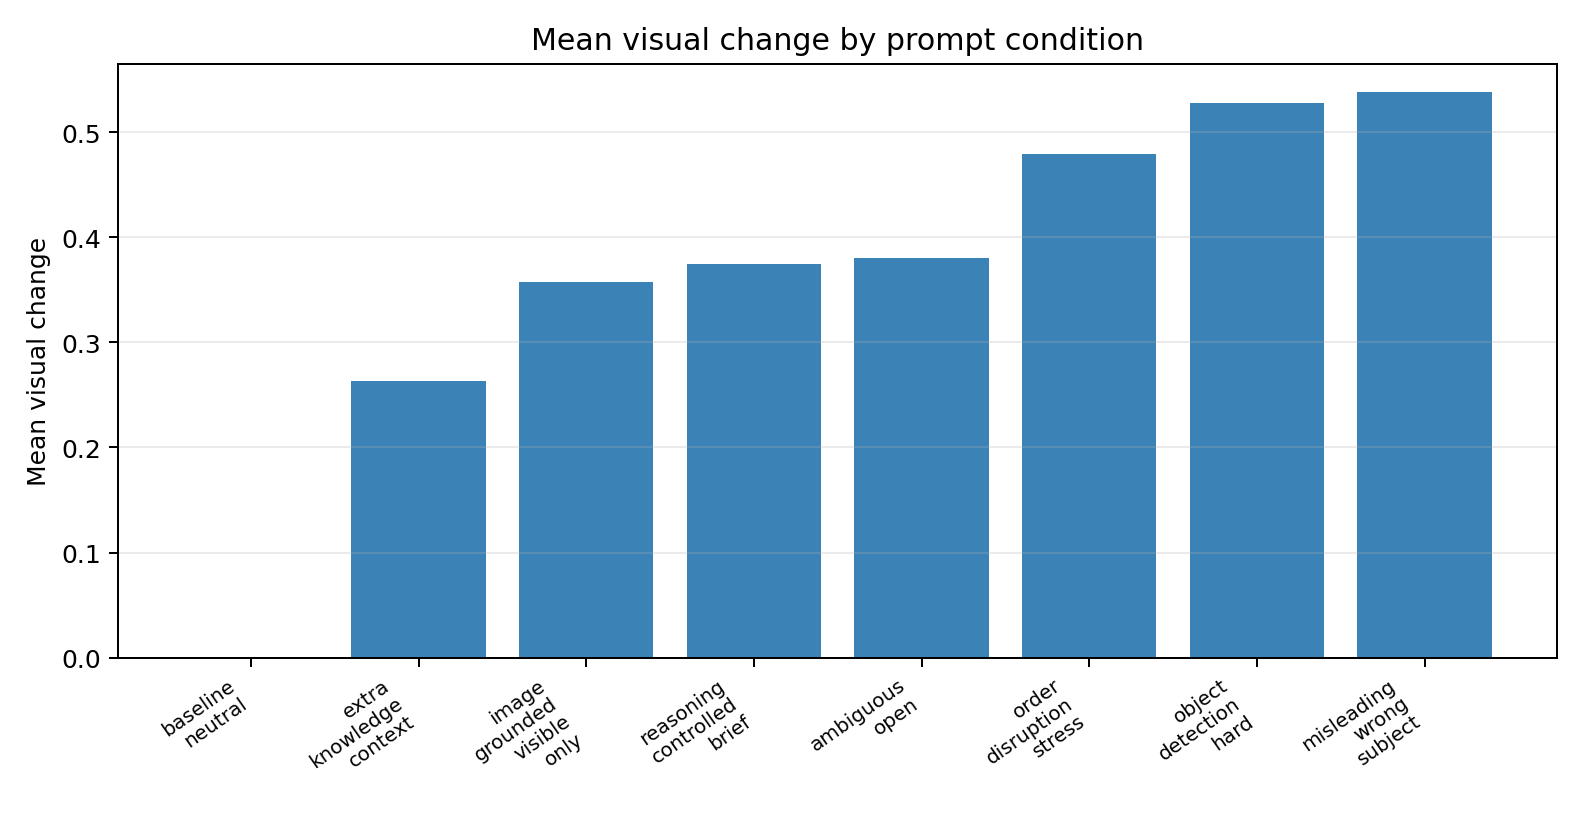
\includegraphics[width=0.96\linewidth]{figures/boxplot_visual_change_by_prompt.png}
\caption{Mean visual change index by prompt condition. The baseline is zero by definition.}
\label{fig:visualchange}
\end{figure}

\FloatBarrier

\subsection{Prompt metric fingerprints}

The effect is not limited to a single composite score. Table~\ref{tab:fingerprint} shows the mean changes, measured relative to the baseline, for representative metric families.

\begin{table}[H]
\centering
\scriptsize
\begin{tabularx}{\linewidth}{>{\ttfamily\scriptsize}Y r r r r}
\toprule
Prompt condition & Entropy $\Delta$ & Top 5 mass $\Delta$ & Effective area $\Delta$ & Centroid shift \\
\midrule
image\_grounded\_visible\_only & 0.0019 & -0.0062 & 0.0108 & 0.1997 \\
ambiguous\_open & -0.0008 & 0.0014 & 0.0119 & 0.1868 \\
misleading\_wrong\_subject & -0.0128 & 0.0427 & -0.0271 & 0.2076 \\
extra\_knowledge\_context & -0.0015 & 0.0055 & -0.0084 & 0.1906 \\
reasoning\_controlled\_brief & -0.0058 & 0.0199 & -0.0216 & 0.2174 \\
order\_disruption\_stress & -0.0011 & 0.0092 & -0.0170 & 0.1990 \\
object\_detection\_hard & -0.0092 & 0.0329 & -0.0258 & 0.1848 \\
\bottomrule
\end{tabularx}
\caption{Compact prompt fingerprint relative to the neutral baseline.}
\label{tab:fingerprint}
\end{table}

The misleading, object detection and brief reasoning conditions tend to produce more concentrated profiles. Entropy decreases, top 5 mass increases and effective area decreases. The prompt constrained to visible details and the ambiguous prompt are comparatively more diffuse. These are average tendencies and do not describe every image in the same way.

\subsection{Prompt separability}

\begin{table}[H]
\centering
\small
\begin{tabularx}{\linewidth}{Y r r r r r}
\toprule
Variant & Cases & Classes & Chance & Balanced accuracy & Macro F1 \\
\midrule
TAM only, baseline excluded & 700 & 7 & 14.3\% & 51.7\% & 50.8\% \\
TAM plus text, baseline excluded & 700 & 7 & 14.3\% & 60.1\% & 58.4\% \\
\bottomrule
\end{tabularx}
\caption{Prompt separability control using five folds grouped by image and a nearest centroid classifier.}
\label{tab:separability}
\end{table}

Both variants perform well above the chance level for seven classes. The TAM only features achieve 51.7\% balanced accuracy, which indicates that the prompt conditions leave distinguishable attribution signatures even without features taken from the response text. Adding output diagnostics increases balanced accuracy to 60.1\%. This shows that response format and textual divergence add useful information. The result does not imply that one prompt is better or more faithful. It only shows that the conditions are separable in the selected metric space.

\begin{figure}[H]
\centering
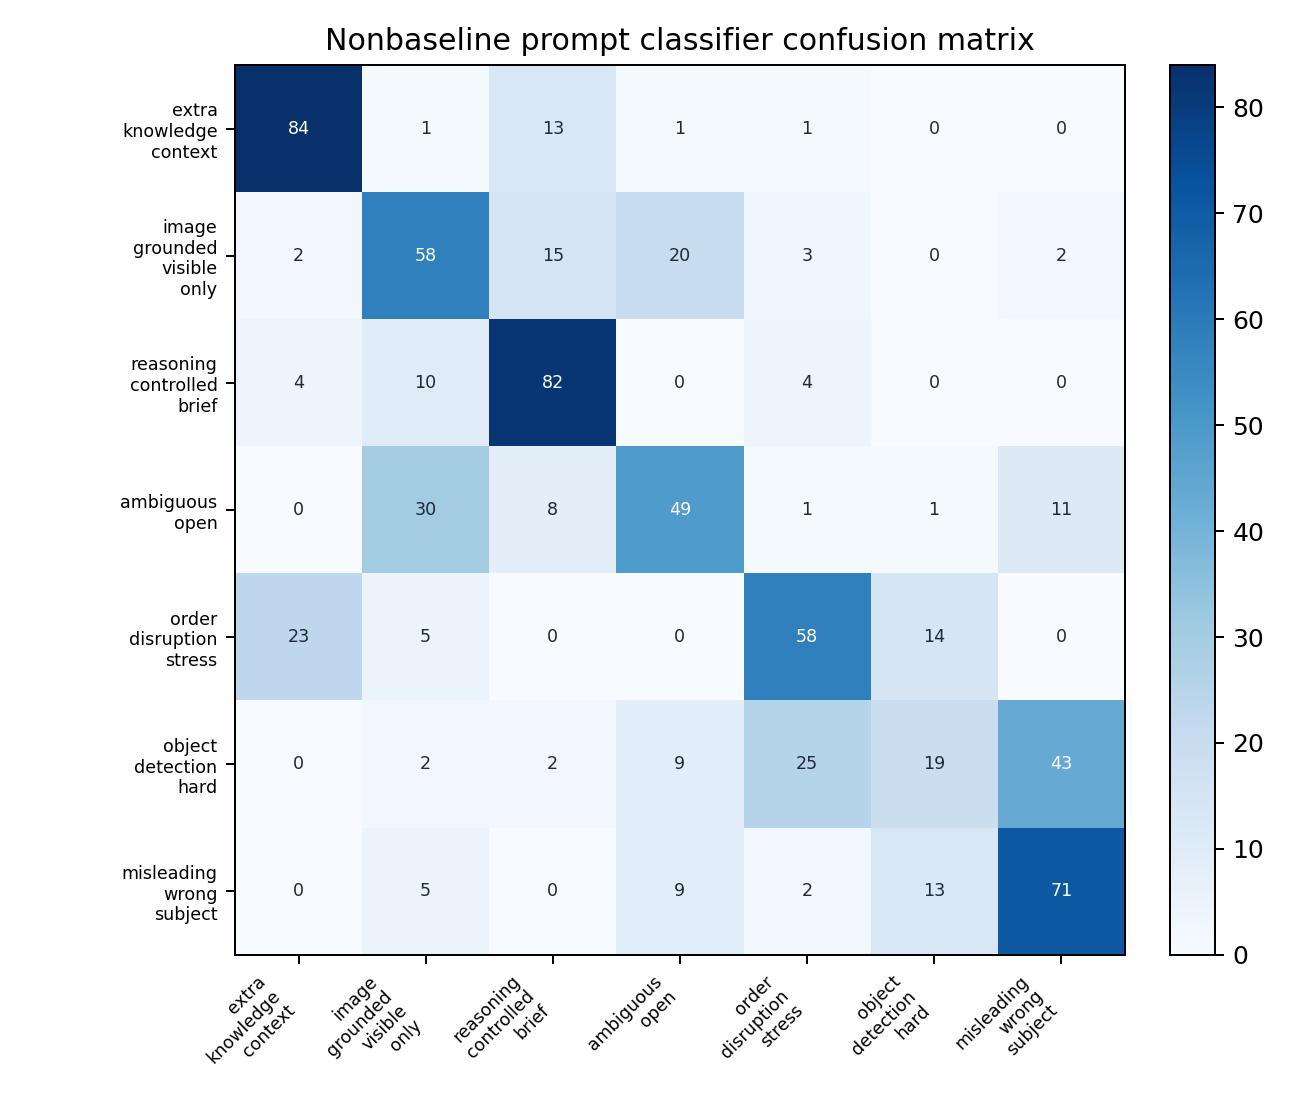
\includegraphics[width=0.79\linewidth]{figures/prompt_classifier_confusion_matrix_nonbaseline.png}
\caption{Confusion matrix for the nearest centroid experiment without the baseline. Each row contains 100 cases.}
\label{fig:confusion}
\end{figure}

The matrix shows that some confusions are more common than others. For example, cases from the object detection prompt are often confused with the misleading prompt or the condition that changes the response order. The prompts that encourage extra knowledge or brief reasoning are more distinctive. These patterns are consistent with overlapping characteristics in the responses and attribution maps rather than with random error.

\FloatBarrier

\subsection{Bounding box and location responses}

Prompt wording strongly affects whether the model produces coordinates or other location information. The strict flag identifies 139 responses with bbox or location signals, while the coordinate parser can render 102 responses as points or rectangular overlays.

\begin{table}[H]
\centering
\small
\begin{tabular}{lrrr}
\toprule
Prompt condition & Strict count & Parseable count & Strict rate \\
\midrule
baseline\_neutral & 9 & 0 & 9\% \\
image\_grounded\_visible\_only & 4 & 0 & 4\% \\
ambiguous\_open & 1 & 0 & 1\% \\
misleading\_wrong\_subject & 2 & 2 & 2\% \\
extra\_knowledge\_context & 6 & 0 & 6\% \\
reasoning\_controlled\_brief & 13 & 0 & 13\% \\
order\_disruption\_stress & 76 & 72 & 76\% \\
object\_detection\_hard & 28 & 28 & 28\% \\
\midrule
Total & 139 & 102 & 17.4\% \\
\bottomrule
\end{tabular}
\caption{Strict bbox or location signals and coordinate patterns that can be parsed into dashboard overlays. The total rate is computed over all 800 cases.}
\label{tab:bbox}
\end{table}

Most parseable outputs come from the condition that changes the response order, with 72 cases, and from the object detection prompt, with 28 cases. The remaining two are produced by the misleading prompt. This concentration shows that some instructions can push the model toward spatial formats that appear precise. It does not show that the predicted regions are correct.

\begin{figure}[H]
\centering
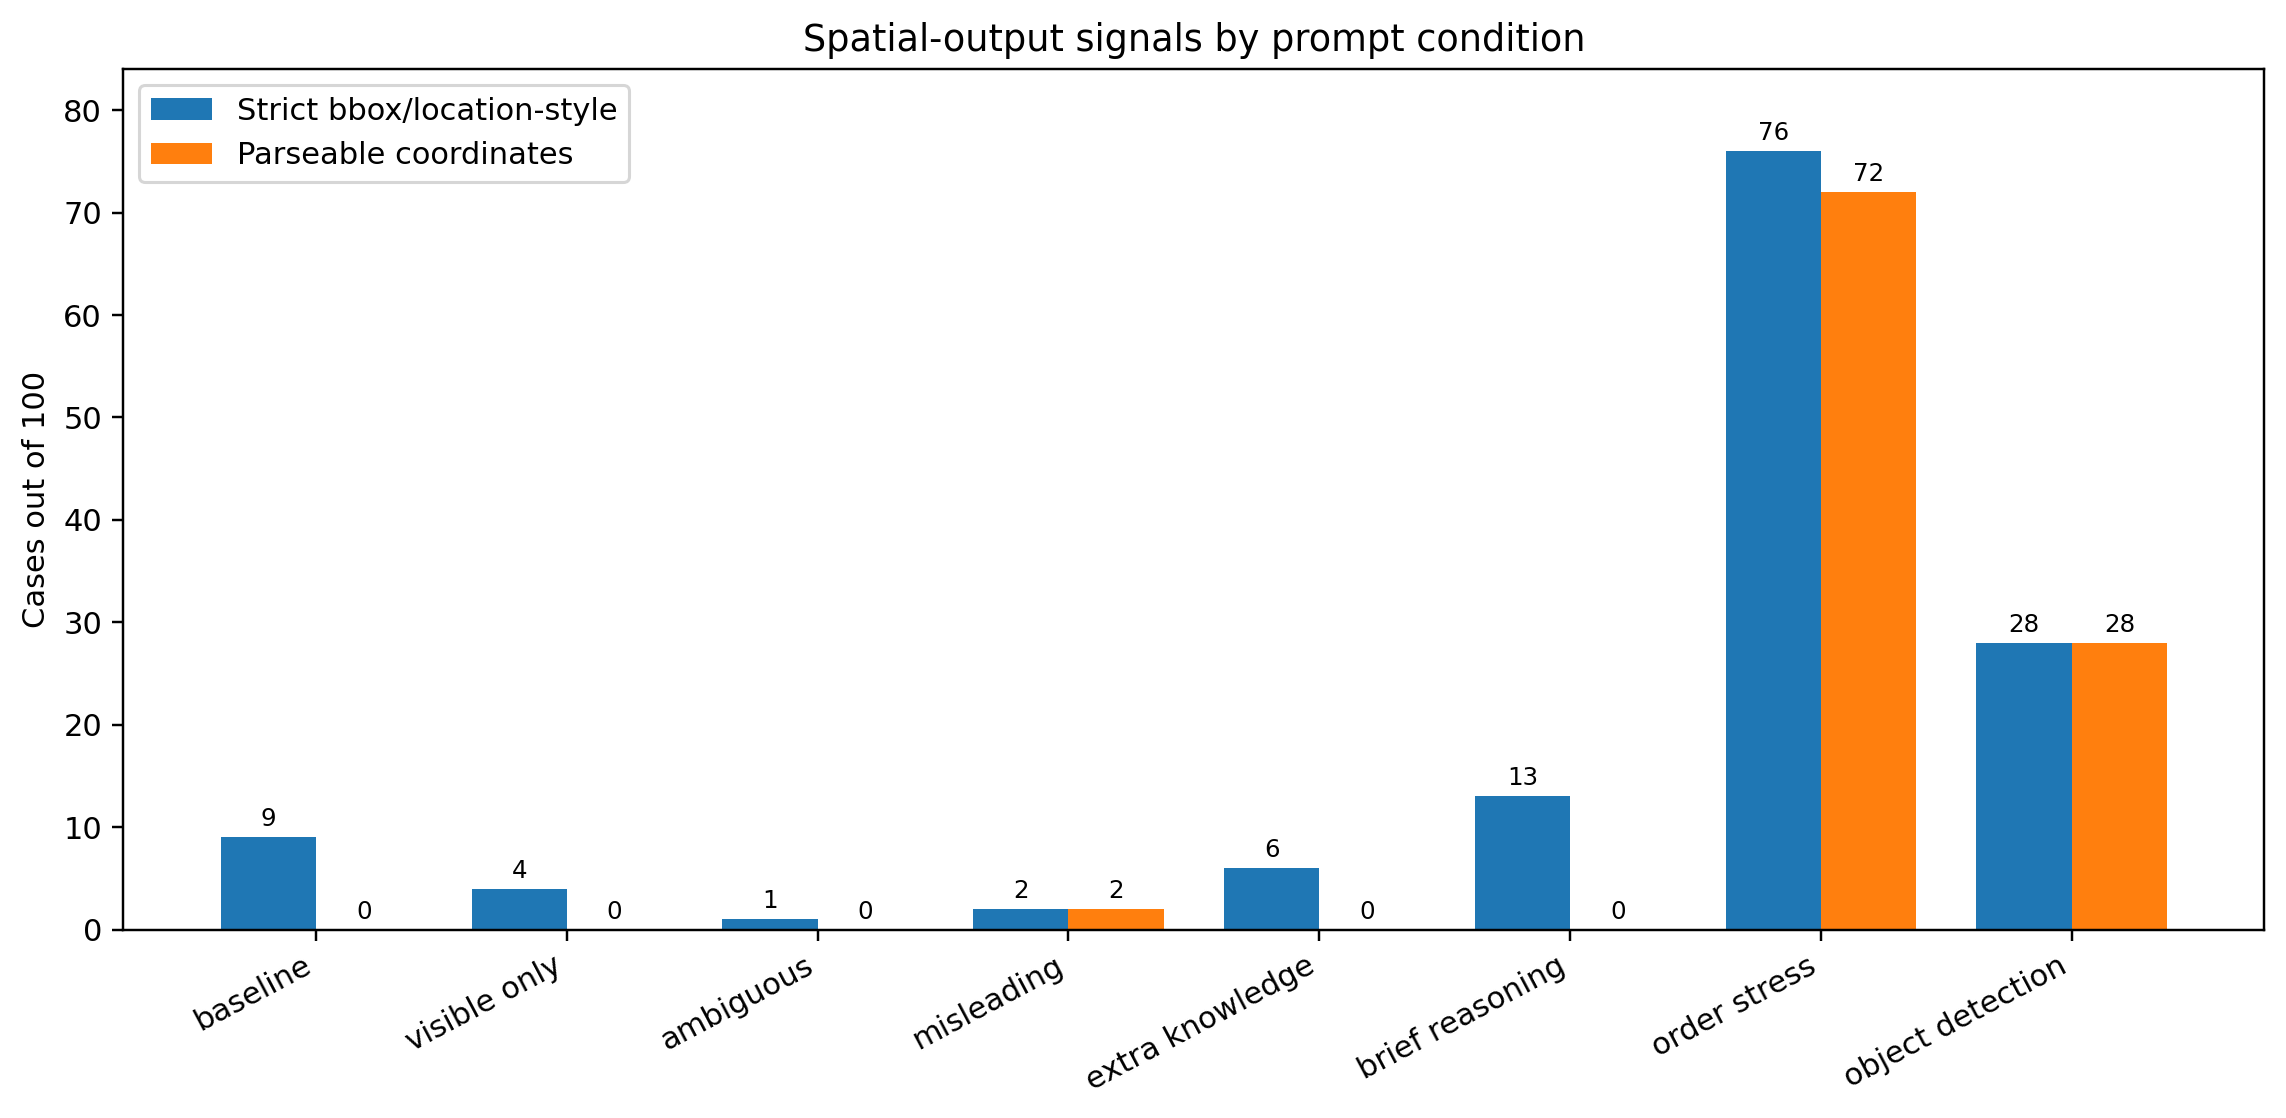
\includegraphics[width=0.98\linewidth]{figures/bbox_style_vs_parseable.png}
\caption{Responses with strict bbox or location signals compared with outputs whose coordinates can be parsed and rendered.}
\label{fig:bbox}
\end{figure}

A response such as \code{a car(153,105),(503,390)} is syntactically parseable as a rectangular region and can therefore be inspected as an overlay. The rectangle must still be compared with the image and available annotations. No IoU, mAP or pointing game score is inferred from parseability alone.

\FloatBarrier

\subsection{Representative diagnostic cases}

The cases in Table~\ref{tab:cases} were selected from the final ranking of cases to illustrate high sensitivity, misleading context and stability under stress. They are examples for qualitative inspection and are not automatically labelled as failures.

\begin{table}[H]
\centering
\scriptsize
\begin{tabularx}{\linewidth}{r >{\ttfamily\scriptsize}p{0.26\linewidth} r Y}
\toprule
COCO image ID & Prompt & Visual change & Diagnostic role \\
\midrule
376284 & order\_disruption\_stress & 0.733 & Highest ranked shift; response includes \code{a car(153,105),(503,390)}, illustrating structured spatial output. \\
018380 & misleading\_wrong\_subject & 0.708 & Strong shift under a misleading prompt; response rejects the requested dog but the attribution still changes substantially. \\
056127 & order\_disruption\_stress & 0.087 & Low change counterexample showing that a stress prompt does not always induce a large shift. \\
\bottomrule
\end{tabularx}
\caption{Representative diagnostic cases from the feature table. COCO file names may contain leading zeros in stored paths.}
\label{tab:cases}
\end{table}

It is important to include both cases with high sensitivity and cases with low sensitivity. Selecting only visually striking failures would exaggerate the effect and hide the fact that prompt sensitivity depends on the interaction between the image and the prompt.

\section{Discussion and Security Implications}

The results support three main observations.

First, response plausibility and attribution stability are different properties. A model can generate fluent text while the spatial distribution associated with generation changes under prompt reformulation. This motivates testing multiple prompt templates rather than validating a multimodal system with a single neutral instruction.

Second, the prompt conditions leave measurable fingerprints. Separability above chance with TAM only features suggests that the effect is not restricted to answer length or formatting. At the same time, the improvement obtained by adding features from the text and output confirms that visual and linguistic behavior are connected.

Third, a structured output should not be confused with verified localization. Of the 139 responses flagged for bbox or location information, 102 contain coordinates that the dashboard can parse and render. This shows that spatial claims which appear precise are common with the prompt that changes response order and with the object detection prompt. However, compatibility with the parser is not the same as localization accuracy. Each overlay still has to be compared with the image and the annotations before it can be considered spatially correct.

From a security perspective, the prompt should therefore be considered part of the system configuration that is being evaluated. User instructions, templates and downstream orchestration can change the context. A robust audit should test whether both outputs and explanation proxies remain stable with plausible, ambiguous and misleading prompts, as well as prompts that impose a specific format.

\section{Limitations}

The study has several limitations.

\begin{itemize}
  \item \textbf{Explanation scope.} TAMs are not ground truth and do not prove causal faithfulness, correct grounding or model intention.
  \item \textbf{Dataset scope.} The final snapshot contains 100 COCO images and one model. The original image selection criterion could not be fully recovered, so broad representativeness is not claimed.
  \item \textbf{Composite score.} \code{visual\_change} is an average of percentile ranks computed within this experimental set. It is useful for ranking and comparison, but it has no absolute physical meaning and mixes multiple feature families.
  \item \textbf{Heuristic regions and trajectories.} Hotspots depend on thresholding and connected components. Scanpaths are derived from TAM centroid trajectories, not human gaze.
  \item \textbf{Location outputs.} Strict bbox or location flags measure response format, while parseable coordinate counts measure compatibility with the overlay parser. Neither evaluates localization accuracy; the COCO comparison remains qualitative and no IoU or mAP benchmark is reported.
  \item \textbf{No causal benchmark.} The report does not include deletion/insertion tests, systematic pointing game evaluation, mass in mask analysis or a full COCO IoU/mAP benchmark.
  \item \textbf{Reproducibility artifacts.} Raw maps, the SQLite database and large exports are maintained outside GitHub because of their size; the repository contains code, configurations and documentation.
\end{itemize}

\section{Conclusion and Future Work}

This project developed a structured pipeline for studying prompt sensitivity in a multimodal model through Token Activation Maps. The analysis covers 800 cases obtained by applying eight prompts to 100 images. The prompt conditions differ in visual change relative to the baseline, concentration, diffusion, spatial displacement, hotspot structure and trajectories based on attribution centroids. A nearest centroid control grouped by image separates the seven prompts other than the baseline well above chance using TAM only features. The result improves further when response diagnostics are added.

The main conclusion is not that TAM proves correct visual grounding. TAM instead provides a practical diagnostic view of how attribution behavior changes when the linguistic context changes. The misleading prompt, the object detection prompt and the prompt that changes response order produce the largest average shifts. These conditions also account for most of the 102 parseable coordinate outputs, showing that the prompt can create an appearance of spatial precision. The presence of stable counterexamples shows that sensitivity still depends on the interaction between the image and the prompt.

Future work should extend the analysis to other models and datasets, preserve an explicit manifest of the selected images, evaluate map faithfulness through perturbation tests and compare TAMs quantitatively with object masks or bounding boxes using clearly defined localization metrics. A compact versioned package with selected cases and dashboard artifacts would also improve reproducibility without requiring distribution of the complete archive of raw maps.

\printbibliography[heading=bibintoc,title={References}]

\end{document}
